% Diapositivas de la réplica. Números: resultados.tex (src/figuras.py).
\begin{frame}{Réplica: el experimento del Apéndice B, a escala de CPU}
  \begin{columns}[T]
    \begin{column}{.5\textwidth}
      \begin{block}{Igual que el artículo}
        \footnotesize
        \begin{itemize}
          \item \textbf{Datos}: CIFAR-10 (Krizhevsky, 2009): \texttt{cs.toronto.edu/\textasciitilde kriz/cifar-10.html}.
          \item Arquitectura: su Fig.~7 literal; los parámetros coinciden con la ec.~(4).
          \item AdamW, tasa triangular, recorte de gradiente, escalado aleatorio, \emph{weight decay} $10^{-2}$.
          \item Comparación con una \textbf{ResNet con la misma receta}, y ablaciones de núcleo y de parche.
        \end{itemize}
      \end{block}
    \end{column}
    \begin{column}{.46\textwidth}
      \begin{alertblock}{Distinto, por cómputo (CPU, sin GPU)}
        \footnotesize
        \begin{itemize}
          \item 10 épocas en lugar de 200.
          \item ConvMixer-128/8, $p=2$ (no 256/8, $p=1$: 3,5\,h \emph{por época}).
          \item Sin RandAugment, mixup ni CutMix.
        \end{itemize}
      \end{alertblock}
      \vspace{3pt}
      \begin{exampleblock}{Más estricto que el artículo (U1)}
        \footnotesize 45\,000 / 5\,000 / 10\,000 (entr./valid./test). Test mirado \textbf{una sola vez}.
      \end{exampleblock}
    \end{column}
  \end{columns}
  \fuente{\textit{Nota.} Código, semillas e hiperparámetros: \texttt{src/}, \texttt{config.json} y \texttt{notebooks/replica\_convmixer.ipynb}.}
\end{frame}

\begin{frame}{Resultado: las CNN quedan muy arriba; ConvMixer y ResNet empatan}
  \begin{columns}[T]
    \begin{column}{.60\textwidth}
      \centering
      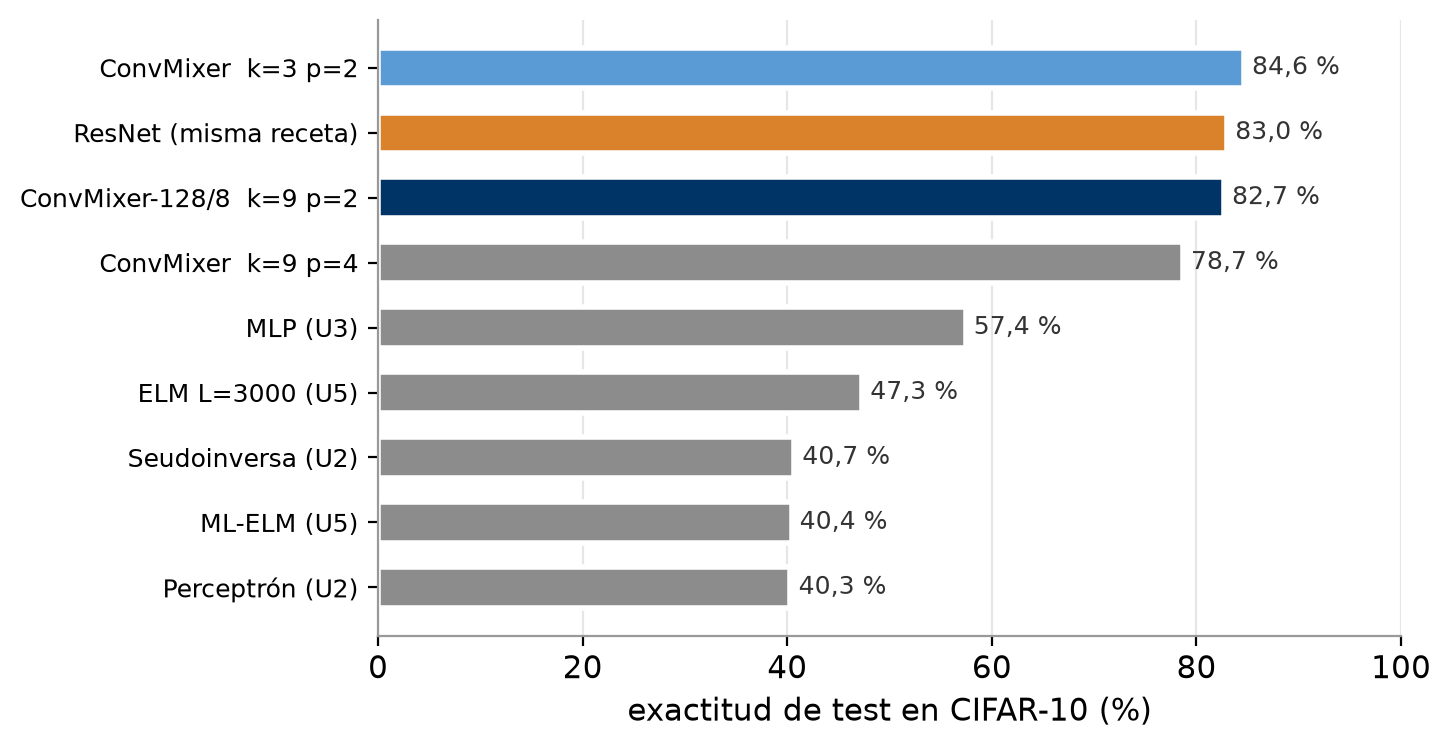
\includegraphics[width=\linewidth,height=0.70\textheight,keepaspectratio]{f_barras.png}
    \end{column}
    \begin{column}{.37\textwidth}
      \footnotesize
      \textbf{ConvMixer-128/8}: \accCMnueve\,\% con \paramsCMnueve{} parámetros.\\
      \textbf{ResNet}, misma receta: \accResNet\,\% con \paramsResNet.\\[4pt]
      El MLP tiene 16 veces más parámetros y queda 25 puntos abajo: lo que importa es el \textbf{sesgo inductivo}
      (localidad y pesos compartidos), no la cantidad de parámetros.\\[4pt]
      Lineales $\approx$ 40\,\%; la ELM mejora con más neuronas, pero sus rasgos aleatorios no ven la geometría
      de la imagen.
    \end{column}
  \end{columns}
  \fuente{\textit{Nota.} Exactitud de test (10\,000 imágenes). Modelos no convolucionales: promedio de 3 semillas. Elaboración propia.}
\end{frame}

\figslide{Curvas de validación: con 10 épocas todos siguen aprendiendo}{f_curvas_validacion.png}{\textit{Nota.} La validación se estabiliza al final porque la tasa de aprendizaje llega a cero, no porque el modelo haya terminado de aprender. Elaboración propia.}

\begin{frame}{Ablaciones frente a la Tabla 4: qué se reprodujo y qué no}
  \begin{columns}[T]
    \begin{column}{.55\textwidth}
      \centering
      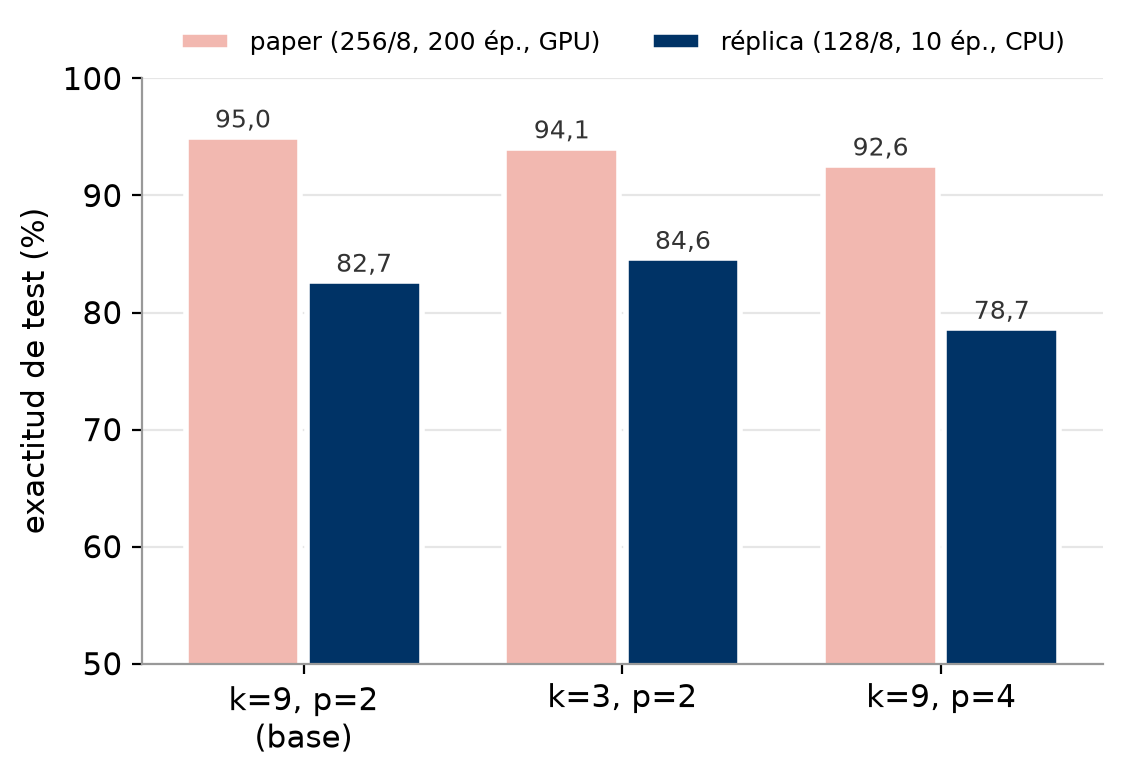
\includegraphics[width=\linewidth,height=0.66\textheight,keepaspectratio]{f_ablaciones.png}
    \end{column}
    \begin{column}{.42\textwidth}
      \footnotesize
      \textbf{Parche: se reproduce.} $p=4$ pierde \difPatch{} puntos (paper: 2,4). Menos resolución interna,
      menos detalle.\\[5pt]
      \textbf{Núcleo: no se reproduce.} $k=3$ \emph{gana} por \difKernelAbs{} puntos. Con pocas épocas converge antes
      el modelo más simple; los autores mismos dicen que el efecto de $k$ grande podría depender de entrenar más.
      Una sola semilla: indicativo, no concluyente.\\[5pt]
      \textbf{ConvMixer vs.\ ResNet}: 0,3 puntos, dentro del ruido. La ventaja del paper aparece en ImageNet con
      modelos 100 veces más grandes.
    \end{column}
  \end{columns}
  \fuente{\textit{Nota.} Réplica: ConvMixer-128/8, 10 épocas, CPU. Artículo: ConvMixer-256/8, 200 épocas, GPU (Trockman y Kolter, 2023, Tabla 4).}
\end{frame}

\begin{frame}{El costo sí se reproduce: el ConvMixer es lento}
  \begin{columns}[T]
    \begin{column}{.56\textwidth}
      \centering
      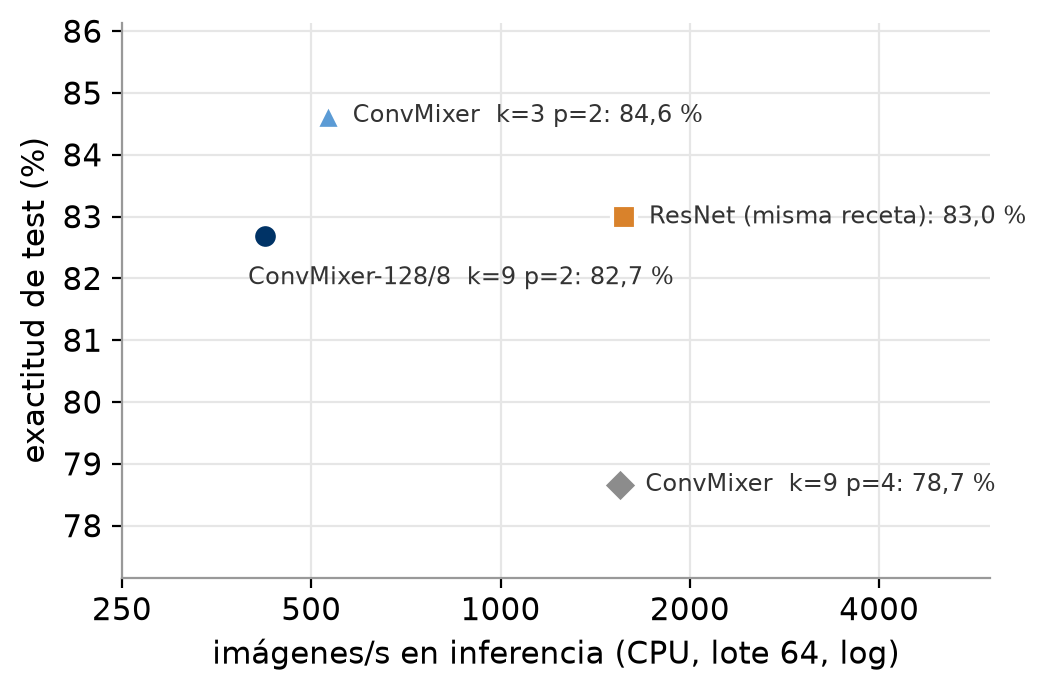
\includegraphics[width=\linewidth,height=0.68\textheight,keepaspectratio]{f_throughput.png}
    \end{column}
    \begin{column}{.40\textwidth}
      \bignum{\ratioTput$\times$}{más rápida la ResNet en inferencia\\(\tputResNet{} frente a \tputCMnueve{} imágenes/s en CPU)}
      \vspace{8pt}
      {\footnotesize Entrenamiento: 110 min el ConvMixer, 32 min la ResNet. La convolución depthwise de núcleo
      grande sobre una resolución interna alta está poco optimizada, igual que lo admiten los autores (Tablas 1 y 2).}
    \end{column}
  \end{columns}
  \fuente{\textit{Nota.} Lote de 64 imágenes, misma CPU de 8 núcleos, eje logarítmico. Elaboración propia.}
\end{frame}

\begin{frame}{¿Y si le doy el cómputo del paper? Réplica en GPU (Google Colab)}
  \begin{columns}[T]
    \begin{column}{.58\textwidth}
      \centering
      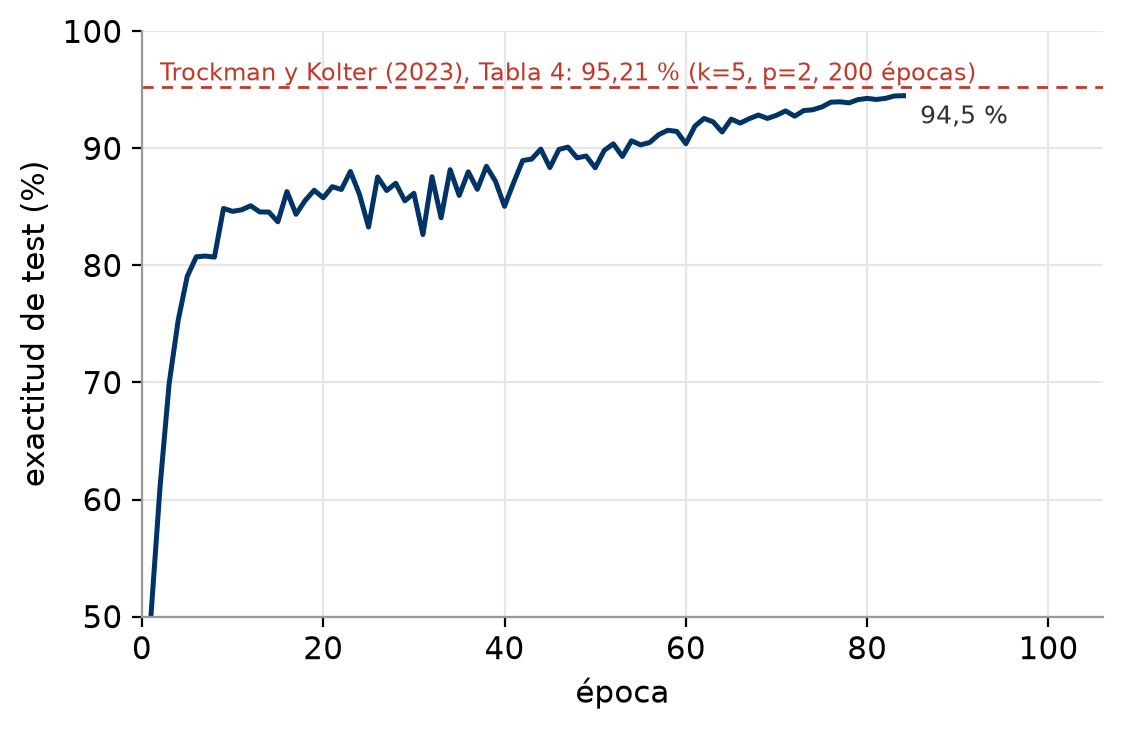
\includegraphics[width=\linewidth,height=0.66\textheight,keepaspectratio]{f_colab.png}
    \end{column}
    \begin{column}{.39\textwidth}
      \bignum{\accColab\,\%}{ConvMixer-256/8, $k=5$, $p=2$, receta oficial de los autores\\(paper: 95,21\,\%)}
      \vspace{6pt}
      {\footnotesize GPU T4 gratuita, unos \segColab{} s por época con RandAugment, ColorJitter y \emph{random
      erasing}. La brecha de la réplica en CPU se explica por la escala, no por la implementación.}
    \end{column}
  \end{columns}
  \fuente{\textit{Nota.} Receta de \texttt{github.com/locuslab/convmixer-cifar10} (Trockman y Kolter, 2023). Se informa la última época, \colabNota.}
\end{frame}

\begin{frame}{CPU frente a GPU: el cómputo y la receta pesan más que la arquitectura}
  \centering\footnotesize
  \resizebox{\linewidth}{!}{\begin{tabular}{lcccc}
    \toprule
     & \textbf{CPU propia} & \textbf{Colab (T4)} & \textbf{Kaggle (T4)} & \textbf{Artículo (GPU)}\\
    \midrule
    Modelo & 128/8, $k$=9, $p$=2 & 256/8, $k$=5, $p$=2 & 256/8, $k$=5, $p$=2 & 256/8, $p$=2\\
    Parámetros & 223\,k & 594\,k & 594\,k & 709\,k / 594\,k\\
    Receta & escalado, recorte, espejo & + RandAugment, borrado & + mixup, CutMix, wd 0 & \texttt{timm} + mixup, CutMix\\
    Épocas & \epocasCNN & \epColab & \epKaggle & 200\\
    Tiempo por época & \minEpCPU{} min & \segColab{} s & \segKaggle{} s & --\\
    Tiempo total & \minCMnueve{} min & \minColab{} min & \minKaggle{} min & --\\
    \rowcolor{unajgris}\textbf{Exactitud de test} & \textbf{\accCMnueve\,\%} & \textbf{\accColab\,\%} & \textbf{\accKaggle\,\%} & \textbf{95,0 / 95,21\,\%}\\
    \bottomrule
  \end{tabular}}
  \vspace{6pt}
  \begin{columns}[T]
    \begin{column}{.48\textwidth}\footnotesize
      \textbf{Lectura}: con la receta del artículo (200 épocas, mixup, CutMix) la réplica \textbf{iguala} el valor
      publicado: \accKaggle\,\% frente a 95,21\,\%. Con una sola semilla, los 0,27 puntos de diferencia no
      son una mejora demostrada.
    \end{column}
    \begin{column}{.48\textwidth}\footnotesize
      \textbf{Para el debate}: Kaggle fue más del doble de rápido por época con la misma GPU (no sé a qué se debe).
      Colab nos negó la GPU por límite de uso y cortó una corrida en la época 84. ¿Cuánto de ``el mejor modelo'' es
      ``el que más cómputo recibió''?
    \end{column}
  \end{columns}
  \fuente{\textit{Nota.} Una corrida por configuración. Se informa la última época. Valores del artículo: Trockman y Kolter (2023, Tabla 4). Elaboración propia.}
\end{frame}

